% SC4012 --- Chapter 1: Threat Modeling, STRIDE, Attack Trees (0->100 ground-up)
\chapter{Threat Modeling, STRIDE and Attack Trees}
\label{ch:threat}

\begin{quote}
\emph{``You cannot defend what you do not understand.''} --- Threat modeling forces us to draw the system before the attacker does: who wants what, where they can enter, and which failures hurt the most.
\end{quote}

\noindent\fbox{\parbox{\dimexpr\linewidth-2\fboxsep-2\fboxrule}{%
\textbf{From zero: no security background assumed.} We start from everyday reasoning---a house, its doors and valuables---and build the vocabulary of assets, trust boundaries and adversaries. Every term is defined on first use. This chapter is the lens for the whole textbook.}}
\vspace{0.4em}

\section*{Learning Outcomes}
After this chapter you will be able to:
\begin{enumerate}[label=(L\arabic*)]
    \item draw a data-flow diagram with trust boundaries and enumerate entry points;
    \item apply STRIDE to classify threats for each element and interaction;
    \item construct and quantify an attack tree with AND/OR decomposition;
    \item prioritise threats using qualitative risk and DREAD scoring;
    \item propose mitigations that compose (prevent, detect, respond) and argue coverage.
\end{enumerate}

% ============================================================
\section{What Is Threat Modeling?}
\label{sec:what-is-tm}
Intuition first. A house has valuables (jewellery, documents), enclosures (walls, doors), and neighbours with different motives (a curious teenager, a professional burglar, a storm). Security starts by sketching that picture honestly: what is worth stealing, where is the boundary between ``inside'' and ``outside,'' and which doors are actually locked?

Formally, an \emph{asset} is what we protect (data, service, reputation), a \emph{trust boundary} is where privilege or control changes (browser $\to$ server, user $\to$ kernel, process $\to$ database), and a \emph{threat} is a potential event that could harm an asset by exploiting a vulnerability. A \emph{threat actor} is who carries it out; an \emph{attack vector} is how.

\begin{definition}[Threat model]
A \emph{threat model} is a structured description of: (i) system architecture and data flows, (ii) assets and trust boundaries, (iii) threat actors and their capabilities, (iv) enumerated threats per element, and (v) candidate mitigations with residual risk. It is a design artefact, not an afterthought, and it evolves with the system.
\end{definition}

The lightest useful artefact is a \emph{data-flow diagram} (DFD): external entities (rectangles), processes (circles), data stores (open rectangles), and data flows (arrows). Dashed lines mark trust boundaries---every crossing is an attack opportunity.

\begin{figure}[h]\centering
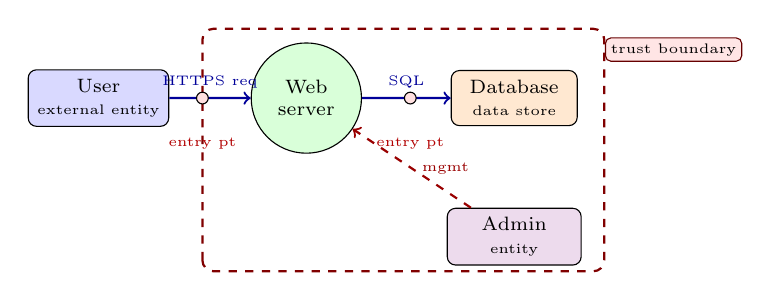
\begin{tikzpicture}[scale=0.88,every node/.style={font=\scriptsize}]
  \node[draw,fill=blue!15,rounded corners=3pt,minimum width=1.7cm,minimum height=0.7cm,align=center] (user) at (-4.5,1.5) {User\\ \tiny external entity};
  \node[draw,fill=green!15,rounded corners=8pt,circle,minimum size=1.4cm,align=center] (web) at (-1.5,1.5) {Web\\server};
  \node[draw,fill=orange!18,rounded corners=3pt,minimum width=1.6cm,minimum height=0.7cm,align=center] (db) at (1.5,1.5) {Database\\ \tiny data store};
  \node[draw,fill=violet!14,rounded corners=3pt,minimum width=1.7cm,minimum height=0.7cm,align=center] (admin) at (1.5,-0.5) {Admin\\ \tiny entity};
  \draw[->,thick,blue!60!black] (user) -- (web) node[midway,above,font=\tiny] {HTTPS req};
  \draw[->,thick,blue!60!black] (web) -- (db) node[midway,above,font=\tiny] {SQL};
  \draw[->,thick,red!60!black,dashed] (admin) -- (web) node[midway,right,font=\tiny] {mgmt};
  \draw[thick,red!50!black,dashed,rounded corners=4pt] (-3.0,-1.0) rectangle (2.8,2.5);
  \node[font=\tiny,fill=red!10,rounded corners=2pt,inner sep=2pt,draw=red!40!black] at (3.8,2.2) {trust boundary};
  \node[draw,fill=red!12,circle,inner sep=1.5pt] (x1) at (-3.0,1.5) {};
  \node[font=\tiny,red!70!black] at (-3.0,0.85) {entry pt};
  \node[draw,fill=red!12,circle,inner sep=1.5pt] (x2) at (0.0,1.5) {};
  \node[font=\tiny,red!70!black] at (0.0,0.85) {entry pt};
\end{tikzpicture}
\caption{Minimal DFD for a web app. The dashed box is the trust boundary (server-side). Red dots are entry points where attacker-controlled data crosses inward; every such crossing invites STRIDE analysis.}
\label{fig:dfd}
\end{figure}

Entry points are where untrusted data enters; assets are where it can cause harm. The modelling question is always: if I were the attacker, which crossing would I choose and what happens if I control what crosses?

\begin{example}[Scope matters]
A file-upload feature adds a new flow \texttt{user $\to$ web $\to$ storage $\to$ rendering}. Without modeling it looks like ``just another form,'' but the DFD reveals three new crossings: upload validation, storage access control, and later rendering in another user's browser (stored XSS). Each needs a threat class.
\end{example}

% ============================================================
\section{STRIDE: Six Threat Classes}
\label{sec:stride}
STRIDE (Microsoft, 1999) gives six buckets that partition most software threats. Mnemonic: each letter is a violation of a security property.

\begin{center}
\small
\begin{tabular}{cllll}
\toprule
Letter & Threat & Violates & Typical element & Example \\
\midrule
S & Spoofing & Authenticity & External entity, process & Fake login page \\
T & Tampering & Integrity & Data flow, store & Modify price in transit \\
R & Repudiation & Non-repudiation & Process & ``I never sent that order'' \\
I & Information disclosure & Confidentiality & Data flow, store & Dump DB via SQLi \\
D & Denial of service & Availability & Process, flow & Flood request queue \\
E & Elevation of privilege & Authorisation & Process & Normal user $\to$ admin \\
\bottomrule
\end{tabular}
\end{center}

Apply STRIDE per DFD element: for each entity ask S/R, for each flow ask T/I/D, for each store ask T/I/D, for each process ask all six. The result is a checklist, not a proof, but a systematic checklist beats ad-hoc brainstorming.

\begin{figure}[h]\centering
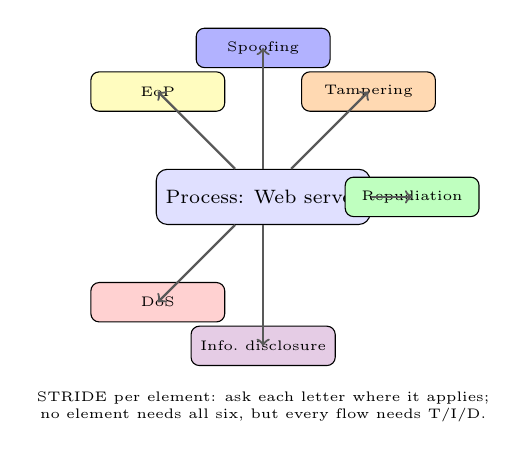
\begin{tikzpicture}[scale=0.86,every node/.style={font=\scriptsize}]
  \node[draw,fill=blue!12,rounded corners=4pt,minimum width=2.4cm,minimum height=0.7cm,align=center] (p) at (0,0) {Process: Web server};
  \foreach \a/\col/\txt in {90/blue!30/Spoofing,45/orange!30/Tampering,0/green!25/Repudiation,270/violet!20/Info.\ disclosure,225/red!18/DoS,135/yellow!25/EoP} {
    \node[draw,fill=\col,rounded corners=3pt,minimum width=1.7cm,minimum height=0.5cm,align=center,font=\tiny] at (\a:2.2) {\txt};
    \draw[->,thick,gray!70!black] (p) -- (\a:2.2);
  }
  \node[font=\tiny,align=center] at (0,-3.1) {STRIDE per element: ask each letter where it applies;\\ no element needs all six, but every flow needs T/I/D.};
\end{tikzpicture}
\caption{STRIDE applied to a single process. Arrows indicate which categories are relevant; colour distinguishes the property violated. Use the DFD to drive the questions.}
\label{fig:stride-process}
\end{figure}

\begin{definition}[STRIDE enumeration]
For a DFD with elements $E$ and flows $F$, define $\text{Threats}(e)\subseteq\text{STRIDE}$ as the subset that can occur at $e$. The model enumerates $\bigcup_{e\in E\cup F}\text{Threats}(e)$ and records for each an attacker capability, impact (CIA), and candidate mitigation.
\end{definition}

\begin{lstlisting}[language=Python]
# STRIDE checklist generator (illustrative enumerator)
DFD_ELEMENTS = {"user": "entity", "web": "process", "db": "store", "flow:user->web": "flow"}
STRIDE_MAP = {
    "entity": ["S","R"], "process": ["S","T","R","I","D","E"],
    "store":  ["T","I","D"], "flow": ["T","I","D"]
}
for elem, kind in DFD_ELEMENTS.items():
    print(elem, ":", ", ".join(STRIDE_MAP[kind]))
# Output: user : S, R  |  web : S, T, R, I, D, E  |  ...
\end{lstlisting}

STRIDE is coarse. It finds categories, not specific exploits; pairing it with attack trees (next) turns ``tampering on the flow'' into a concrete path like ``MITM $\to$ strip TLS $\to$ rewrite price.''

% ============================================================
\section{Attack Trees: From Categories to Paths}
\label{sec:attack-trees}
An \emph{attack tree} (Schneier, 1999) refines a high-level attacker goal into sub-goals connected by AND/OR. OR means any child suffices; AND means all children are needed together. Leaves are atomic attacker actions with a cost or probability; internal nodes compose them.

\begin{definition}[Attack tree]
Root is the attacker's top goal $G$. Children $G_1,\dots,G_k$ are sub-goals with label AND or OR. A cut is a set of leaves whose joint success makes $G$ succeed. Minimal cuts are the smallest such sets; they are the cheapest attack paths.
\end{definition}

\begin{figure}[h]\centering
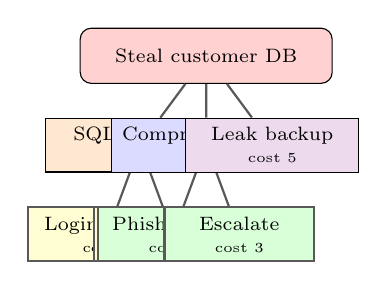
\begin{tikzpicture}[scale=0.84,every node/.style={font=\scriptsize},
  level distance=1.35cm, sibling distance=1.0cm,
  edge from parent/.style={draw,thick,gray!70!black},
  every tree node/.style={draw,rounded corners=3pt,align=center,inner sep=3pt}]
  \node[draw,fill=red!18,rounded corners=4pt,minimum width=3.2cm,minimum height=0.7cm,align=center] {Steal customer DB}
    child {node[draw,fill=orange!18,minimum width=2.4cm,align=center] {SQL injection\\ \tiny OR}
      child {node[draw,fill=yellow!18,minimum width=2.0cm,align=center] {Login bypass\\ \tiny cost 2}}
      child {node[draw,fill=yellow!18,minimum width=2.0cm,align=center] {UNION exfil\\ \tiny cost 3}}
    }
    child {node[draw,fill=blue!14,minimum width=2.4cm,align=center] {Compromise host\\ \tiny AND}
      child {node[draw,fill=green!15,minimum width=1.9cm,align=center] {Phish admin\\ \tiny cost 4}}
      child {node[draw,fill=green!15,minimum width=1.9cm,align=center] {Escalate\\ \tiny cost 3}}
    }
    child {node[draw,fill=violet!14,minimum width=2.2cm,align=center] {Leak backup\\ \tiny cost 5}};
\end{tikzpicture}
\caption{Attack tree for ``steal customer DB.'' OR branches offer alternative paths; the AND branch requires both phishing and escalation. Numbers are illustrative costs; cheapest path is Login bypass (cost 2). Defence prunes cheapest branches first.}
\label{fig:attack-tree}
\end{figure}

Quantification turns the picture into arithmetic. Assign each leaf a cost $c$, success probability $p$, or required skill. Then propagate upward: for AND, $c=\sum c_i$ and $p=\prod p_i$; for OR, $c=\min c_i$ and $p=\max p_i$ (attacker picks the best). The model tells you which branch to harden.

\begin{lstlisting}[language=Python]
# Attack-tree evaluation: minimal cost (AND = sum, OR = min)
tree = {"op": "OR", "children": [
    {"op": "OR", "children": [{"cost":2},{"cost":3}]},
    {"op": "AND","children": [{"cost":4},{"cost":3}]},  # cost 7
    {"cost":5}]}
def min_cost(n):
    if "cost" in n: return n["cost"]
    cs = [min_cost(c) for c in n["children"]]
    return sum(cs) if n["op"]=="AND" else min(cs)
print(min_cost(tree))  # 2 -- the SQLi login bypass dominates
\end{lstlisting}

Risk ties it together. A simple score is $\text{Risk}=\text{Likelihood}\times\text{Impact}$ (low/medium/high or numeric). DREAD refines likelihood into five factors---Damage, Reproducibility, Exploitability, Affected users, Discoverability---each 1--10, averaged. STRIDE finds threats, the attack tree prices them, and risk/DREAD ranks them so mitigations go where they cut the cheapest attack paths first.

\begin{remark}[Threat modelling is iterative]
A model is not a one-time document. Every feature (``add OAuth,'' ``allow file upload'') adds flows and stores; re-run STRIDE on the delta and update the tree. The cheapest path after hardening should be strictly more expensive than before---otherwise the fix was cosmetic.
\end{remark}

% ============================================================
\section{Prioritising Threats: Likelihood, Impact and DREAD}
\label{sec:dread}
Finding thirty threats is easy; fixing them in the right order is the skill. Two complementary lenses are \emph{risk}$=$likelihood$\times$impact and the DREAD average.

Qualitative risk uses a $3\times3$ matrix (low/med/high for each axis). Anything in the high$\times$high corner is fixed before release; low$\times$low can be accepted or logged. Quantitatively, teams score likelihood 1 (needs nation-state) to 10 (script kiddie) and impact 1 (cosmetic) to 10 (full breach), then rank by product.

\begin{figure}[h]\centering
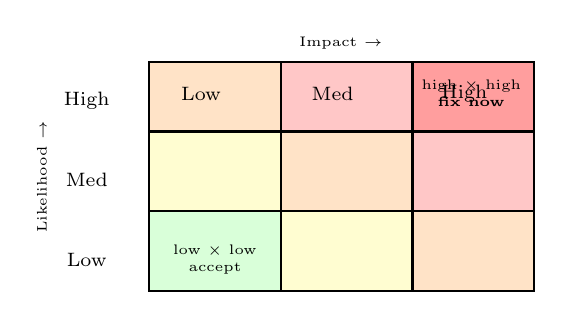
\begin{tikzpicture}[scale=0.88,every node/.style={font=\scriptsize}]
  \fill[green!15] (0,0) rectangle (1.9,1.15);
  \fill[yellow!18] (1.9,0) rectangle (3.8,1.15);
  \fill[orange!22] (3.8,0) rectangle (5.55,1.15);
  \fill[yellow!18] (0,1.15) rectangle (1.9,2.30);
  \fill[orange!22] (1.9,1.15) rectangle (3.8,2.30);
  \fill[red!22] (3.8,1.15) rectangle (5.55,2.30);
  \fill[orange!22] (0,2.30) rectangle (1.9,3.3);
  \fill[red!22] (1.9,2.30) rectangle (3.8,3.3);
  \fill[red!38] (3.8,2.30) rectangle (5.55,3.3);
  \foreach \x/\lab in {0/Low,1.9/Med,3.8/High} \node at (\x+0.75,2.85) {\lab};
  \foreach \y/\lab in {0/Low,1.15/Med,2.30/High} \node at (-0.9,\y+0.45) {\lab};
  \node[font=\tiny,align=center] at (4.65,2.85) {high $\times$ high\\\textbf{fix now}};
  \node[font=\tiny,align=center] at (0.95,0.45) {low $\times$ low\\accept};
  \draw[thick,black] (0,0) rectangle (5.55,3.3);
  \draw[thick] (1.9,0) -- (1.9,3.3); \draw[thick] (3.8,0) -- (3.8,3.3);
  \draw[thick] (0,1.15) -- (5.55,1.15); \draw[thick] (0,2.30) -- (5.55,2.30);
  \node[font=\tiny,above] at (2.77,3.35) {Impact $\to$}; \node[font=\tiny,rotate=90] at (-1.55,1.65) {Likelihood $\to$};
\end{tikzpicture}
\caption{Risk heatmap. Colour deepens toward the top-right where likelihood and impact are both high. DREAD refines the likelihood axis into five scored factors.}
\label{fig:risk-heatmap}
\end{figure}

DREAD scores Damage, Reproducibility, Exploitability, Affected users and Discoverability each $1$--$10$; the average is the priority. Modern teams often replace Discoverability with business impact or map DREAD to CVSS (Ch.~8), but the habit is the same: score openly, rank, and spend engineering where the cheapest path is most damaging.

A mitigation should \emph{prune} a branch of the attack tree, not just obscure it. Prefer eliminating an entry point, then enforcing a property (authentication, integrity check, sandbox), then detecting and recovering. Defence in depth means the attacker must defeat several independent mitigations to reach the asset.

\begin{remark}[Living model]
Every design review starts with ``has the DFD changed?'' A new SDK, a debug endpoint left enabled, or a cache added for performance all add flows and stores. If the model does not evolve, it becomes fiction while the system becomes vulnerable.
\end{remark}

% ============================================================
\section{Exercises}
\label{sec:ch01-exercises}
\begin{enumerate}[label=E1.\arabic*, leftmargin=*, itemsep=0.6em]
    \item \textbf{DFD and boundaries.} Draw a DFD for a chat app (mobile client $\to$ API gateway $\to$ message service $\to$ DB, plus push notification to recipient). Mark trust boundaries and list every entry point where untrusted data crosses inward. Which crossing has highest asset exposure?
    \item \textbf{STRIDE per element.} For the upload flow \texttt{client $\to$ API $\to$ object store $\to$ CDN $\to$ victim browser}, enumerate STRIDE threats at each step. Give one concrete exploit per letter that actually applies (omit letters that do not).
    \item \textbf{Attack tree construction.} Root goal: ``forge admin session.'' Decompose into at least two OR branches (e.g., credential theft vs.\ token forgery) and one AND branch (e.g., XSS + steal cookie + replay). Label leaves with cost 1--5 and compute minimal cost and minimal cut.
    \item \textbf{DREAD scoring.} Score two threats---(a) reflected XSS on search and (b) unauthenticated DB backup download---on each DREAD factor 1--10. Compute averages and rank. Does the ranking match intuition? What would change the order?
    \item \textbf{Mitigation coverage.} Propose one mitigation per STRIDE letter for a login endpoint (e.g., S $\to$ MFA, T $\to$ TLS, etc.) and argue which attack-tree branch each prunes. Identify one residual risk that remains even after all six mitigations.
\end{enumerate}

\section*{Chapter Notes}
STRIDE originates from Microsoft's Trustworthy Computing (Kohnfelder \& Garg, 1999; Shostack, \emph{Threat Modeling: Designing for Security}, 2014). Attack trees are from Schneier (Dr.\ Dobb's, 1999) and formalised in Mauw \& Oostdijk. DFD-based modelling is systematised in OWASP Threat Modeling Cheat Sheet and NIST SP 800-154. For risk, see OWASP Risk Rating and DREAD (now often replaced by CVSS, covered in Ch.~8).

% End of Chapter 1
